%!TEX root = ./main.tex

% content goes here 

\section{Wat is DOT language?}
\begin{frame}
	\frametitle{Wat is DOT language?}
    \begin{itemize}
    \item Wat?
        \begin{itemize}
          \item "Simpele" taal om grafen te visualizeren.
          \item Layout wordt geregeld voor jou (maar je kan ook zelf specifieke wijzigingen maken).
    	\end{itemize}
    \item Waarom?
        \begin{itemize}
          \item Wordt veel gebruikt bij de toepassingsopdrachten van vakken gegeven door Prof. Laenens.
          \item Studenten kijken er initieel enorm tegenop, maar zeggen achteraf dat het wel een goed hulpmiddel is.
    	\end{itemize}
    \item Wat win je door DOT te gebruiken? TIJD!
    	\begin{itemize}
          \item Je kan snel nakijken of je algoritmes correct werken. Noodzakelijk bij verdere Laenens vakken waar je automaten minimaliseert, etc.
    	\end{itemize}
    \end{itemize}
\end{frame}

\section{Voorbeelden}

\defverbatim\lstI{
\begin{lstlisting}[basicstyle=\ttfamily]
graph G {
    A -- B
}
\end{lstlisting}
}

\defverbatim\lstII{
\begin{lstlisting}[basicstyle=\ttfamily]
digraph G {
    A -> B
}
\end{lstlisting}
}

\defverbatim\lstIII{
\begin{lstlisting}[basicstyle=\ttfamily]
graph G {
	node1 [label="A", shape=Mrecord]
	node2 [label="B", shape=record]
	node3 [label="C", shape=circle]
	node4 [label="D"]
}
\end{lstlisting}
}

\defverbatim\lstIIII{
\begin{lstlisting}[basicstyle=\ttfamily]
graph G {
	node1 [label="A", color=Red]
	node2 [label="B", fontcolor=Green]
	node1 -- node2 [label="label", 
  			color=Orange,
                    	fontcolor=Blue]
}
\end{lstlisting}
}

\defverbatim\lstV{
\begin{lstlisting}[basicstyle=\ttfamily]
graph G {
	node1 [label="A"]
	node2 [label="B", style=invis]
	node1 -- node2
}
\end{lstlisting}
}

\defverbatim\lstVI{
\begin{lstlisting}[basicstyle=\ttfamily]
graph G {
	node1 [label="A"]
	node2 [label="B"]
	node1 -- node2
	rankdir=LR;
}
\end{lstlisting}
}

\defverbatim\lstVII{
\begin{lstlisting}[basicstyle=\tiny]
digraph g {
    node [shape=record]
    node0 [label="3|5|8", shape=Mrecord]
    node1 [label="<here> 0|1|2"]
    node2 [label="4", fontcolor=Green]
    node3 [label="7",shape=circle]
    node4 [label="9|20"]

    node0 -> node1:here [color=Red]
    node0 -> node2 [style=invis]
    node0 -> node3 
    node0 -> node4 [label=Go]
    node4 -> "7"
    "7" -> Hey [label="Hello World!", fontcolor=Blue]
    Hey -> Hey [label="a\nb\nc"]

    rankdir=LR;
}
\end{lstlisting}
}

\begin{frame}
	\frametitle{Basic Graaf}
	\lstI
    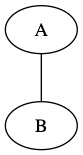
\includegraphics[align=c, width=1.2cm]{res/basic1}
\end{frame}

\begin{frame}
	\frametitle{Soorten}
    \begin{multicols}{2}
    [
    Men kan verschillende soorten grafen tekenen, de gerichte en ongerichte grafen zullen jullie het meest gebruiken:
    ]
    \lstI
    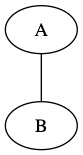
\includegraphics[align=c, width=1.2cm]{res/basic1}
    \newline
    \lstII
    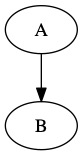
\includegraphics[align=c, width=1.2cm]{res/basic2}
    \end{multicols}
\end{frame}

\begin{frame}
	\frametitle{Vorm}
    \lstIII
    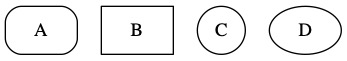
\includegraphics[align=c, width=10cm]{res/basic3}
\end{frame}

\begin{frame}
	\frametitle{Kleur}
    \lstIIII
    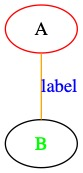
\includegraphics[align=c, width=1.8cm]{res/basic4}
\end{frame}

\begin{frame}
	\frametitle{Zichtbaarheid}
    \lstV
    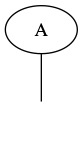
\includegraphics[align=c, width=1.8cm]{res/basic5}
\end{frame}

\begin{frame}
	\frametitle{Richting}
    \lstVI
    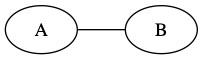
\includegraphics[align=c, width=5.8cm]{res/basic6}
\end{frame}

\begin{frame}
	\frametitle{Extra Documentatie}
    \url{https://www.tonyballantyne.com/graphs.html}
    \url{https://www.graphviz.org/doc/info/lang.html}
    \url{https://graphs.grevian.org/example}
    \url{https://renenyffenegger.ch/notes/tools/Graphviz/examples/index}
\end{frame}

\section{Oefening}
\begin{frame}
	\frametitle{Oefening}
	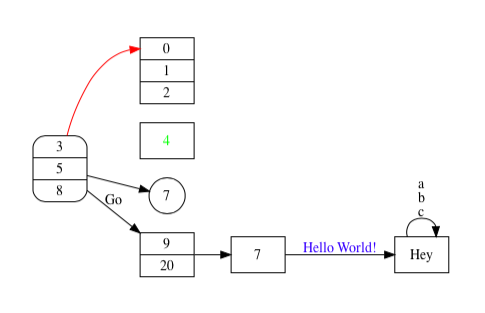
\includegraphics[width=10cm]{res/Dot_Oef}
\end{frame}

\section{Oplossing}
\begin{frame}
	\frametitle{Oplossing}
	\lstVII
\end{frame}